\section*{Cahier des charges}
\addcontentsline{toc}{section}{\protect\numberline{}Cahier des charges}

Même si une très grande liberté nous était laissée dans le cadre de ce projet, le sujet nous imposait quelques éléments.\\

Ainsi, le programme à développer devait posséder une architecture de type \textit{client}/\textit{serveur}, et être capable de fonctionner sur des machines différentes. La communication nécessaire entre les différents composants du programme devait donc reposer sur des échanges entre sockets.

De plus, la partie communication entre les sockets devait être codée en \texttt{langage C}. Cette contrainte avait pour but de nous faire manipuler les sockets à bas niveau, afin de bien comprendre leur fonctionnement.\\

Deux versions du programme étaient demandées, l'une fonctionnant selon le modèle \texttt{1 client/1 serveur}, l'autre selon le modèle \texttt{n clients/1 serveur}. Nous avons cependant choisi d'ignorer cette contrainte, comme nous l'expliquerons dans la partie consacrée à nos choix d'implémentation.

\section*{Fonctionnalités du logiciel}
\addcontentsline{toc}{section}{\protect\numberline{}Fonctionnalités du logiciel}

Comme nous l'avons annoncé dans l'introduction, le programme réalisé dans le cadre de ce projet est inspiré du jeu \textsc{Bomberman} \footnote{\url{http://fr.wikipedia.org/wiki/Bomberman}}. Bien qu'ayant donné lieu à énormément d'adaptations et de copies, le jeu original est sorti en 1983. Il a été développé par \textit{Hudson Soft} et édité par \textit{Konami}.\\

Les règles de notre version sont très simples:
\begin{itemize}
	\item 2 à 4 joueurs s'affrontent sur une carte quadrillée de 9x9 cases, certaines libres, certaines contenant des obstacles.
    \item Le jeu se déroule au tour par tour, ce qui signifie qu'un joueur doit attendre que tous les autres aient joué avant de pouvoir effectuer une action.
    \item Lors de son tour, un joueur peut se déplacer vers une case libre adjacente ou poser une bombe.
    \item Chaque joueur peut avoir 3 bombes posées simultanément sur le terrain.
    \item Une bombe explose après que le joueur l'ayant posée ait joué 6 tours. Tous les joueurs situés dans le rayon de l'explosion (y compris le joueur ayant posé la bombe) perdent 1 point de vie.
    \item Chaque joueur démarre avec 2 points de vie.
    \item La partie se termine lorsqu'un seul joueur possède au moins 1 point de vie.
\end{itemize}

\section*{Choix d'implémentation}
\addcontentsline{toc}{section}{\protect\numberline{}Choix d'implémentation}

Afin de donner un sens à l'architecture \textit{client}/\textit{serveur} imposée, nous avons décidé d'effectuer toute la logique de la partie du côté du serveur. Le client a donc pour seul but de récupérer les actions de l'utilisateur, puis d'afficher les différents états du jeu qui lui sont communiqués.

De plus, le serveur a été conçu de façon à pouvoir gérer plusieurs parties simultanées, comme on peut s'y attendre dans le cadre d'un jeu en réseau.\\

Initialement prévu pour être joué en temps réel (tous les joueurs effectuant leurs actions en même temps), le protocole UDP a été choisi pour la communication \textit{client}/\textit{serveur}.

Ce choix a été fait de part la nature du protocole, qui offre une communication en mode déconnecté. Ce type de connexion permet d'avoir une meilleur vitesse d'échange de messages qu'avec une connection en mode connecté telle que présente avec le protocole TCP. En revanche, aucune garantie n'est présente concernant la façon dont les différents messages seront délivrés (ordre, intégrité, \dots).\\

Ce manque de garantie ne représente cependant pas vraiment un handicap pour un jeu temps réel. En effet, si une action d'un joueur est ponctuellement perdue, les conséquences sur la partie ne sont pas graves.

Cependant, faute de temps pour mettre un tel système en place, nous avons dû modifier nos plans et passer à un jeu en tour par tour. La perte d'une action devient dans cette situation beaucoup plus grave, puisqu'elle bloque complètement la partie.

Dans ces conditions, la communication via le protocole TCP serait donc plus adaptée, mais le temps nous a manqué pour effectuer les changements nécessaires.\\

Compte tenu de la nature de notre application, nous avons également décidé de ne pas réaliser de version 1 client/1 serveur.

En effet, cette version aurait nécessité la mise au point d'une intelligence artificielle pouvant servir d'adversaire. Lui faire faire une action aléatoire à chaque tour n'est pas long à mettre en place, mais n'aurait pas d'intérêt. En effet, il aurait toutes les chances de se suicider en faisant des allers-retours sur ses propres bombes, entraînant sa mort avant même que le joueur ne l'atteigne.

Ne disposant pas du temps nécessaire à l'élaboration d'un ennemi plus performant, nous nous sommes donc concentré sur la version n clients/1 serveur.


\section*{Dépendances externes}
\addcontentsline{toc}{section}{\protect\numberline{}Dépendances externes}

En plus de la bibliothèque standard \texttt{C}, nous avons décidé d'utiliser la \texttt{CSFML} pour mettre en place l'affichage du jeu et la communication entre les sockets.

La \texttt{CSFML} est le binding \texttt{C} officiel de la \texttt{SFML}, une bibliothèque destinée au langage \texttt{C++} conçue pour faciliter la création d'applications multimédia. La version que nous avons choisi d'utiliser est la 1.6. Ce choix s'explique par sa présence dans les dépôts Ubuntu (système linux utilisé pour développer le logiciel), ce qui facilite son installation.

\section*{Interface graphique}
\addcontentsline{toc}{section}{\protect\numberline{}Interface graphique}

Dans le but d'offrir à l'utilisateur principal (le client) un rendu clair et agréable, nous avons opté pour une interface graphique plutôt qu'un affichage dans une console.

Celle-ci a été entièrement construite avec la \texttt{CSFML}, et est composée d'un ensemble d'éléments graphiques, appelés \textit{sprites} placés sur une grille.

Nous avons créé l'intégralité de nos sprites nous même à l'aide d'une base de donnée d'images libres et d'un logiciel infographique. \\

\noindent{Voici quelques exemples de sprites : \\
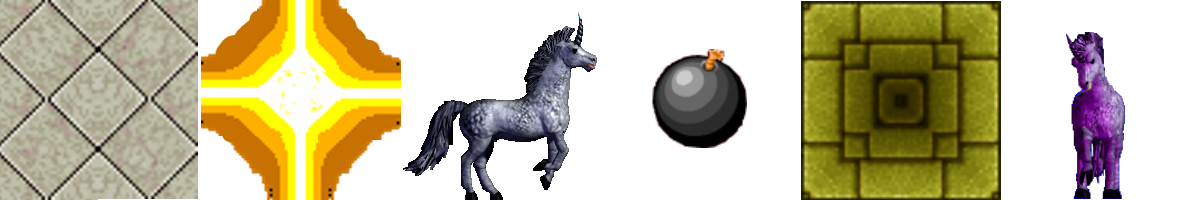
\includegraphics[width=1\textwidth]{Figures/exempleSprite.png}}\\

\noindent{Voici la carte créée avec les sprites : \\
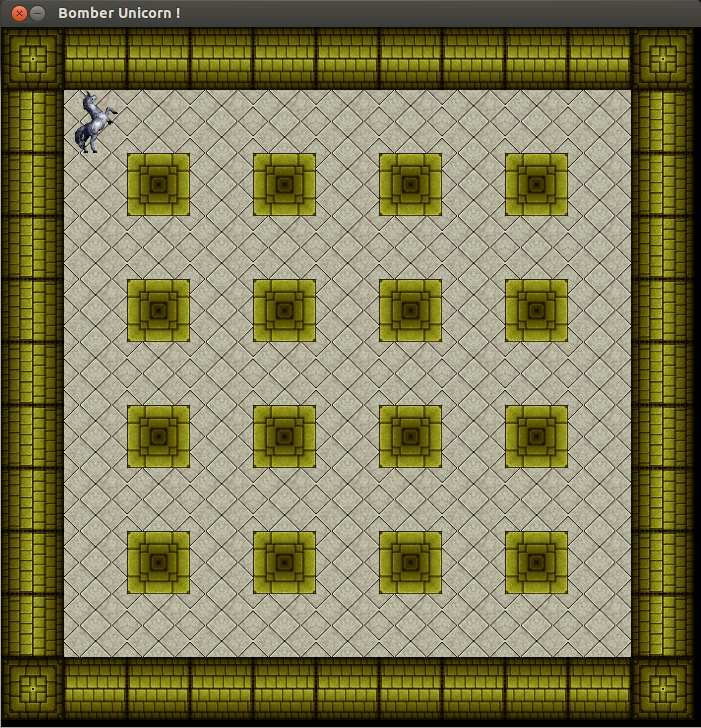
\includegraphics[width=0.9\textwidth]{Figures/mapSprite.png}}


